\begin{align*}
    \boldsymbol{n} &= \begin{bmatrix}
        -1 \\ 1
    \end{bmatrix} \\
    \boldsymbol{z} &= \begin{bmatrix}
        -1 \\ 1.01
    \end{bmatrix} \\
    \boldsymbol{S} &= \begin{bmatrix}
        2 & 1 \\
        1 & 2
    \end{bmatrix}
\end{align*}

On the same axes, plot the vectors $\boldsymbol{n}$ and $\boldsymbol{z}$ using MATLAB.

\begin{solution} \
    \begin{lstlisting}[language=Matlab]
n = [-1; 1];
z = [-1; 1.01];

hold on
quiver(0, 0, n(1), n(2));
quiver(0, 0, z(1), z(2));

legend('n', 'z')
    \end{lstlisting}
    \begin{center}
        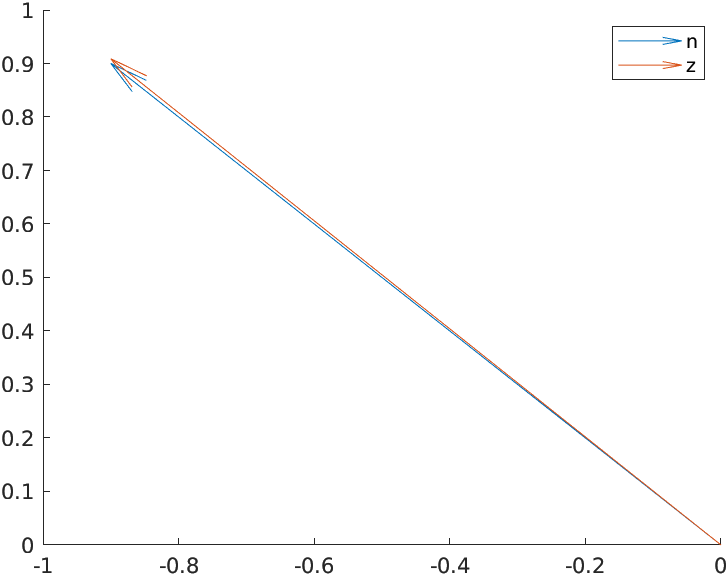
\includegraphics[width=0.7\textwidth]{img/e8p1.png}
    \end{center}
\end{solution}